\chapter*{Reflecting on rules and examples}

\ifnotes

    Before starting ask "Which is more important, Rules or Examples?" Answer is they go together. Neither is more important than the other.
    
    Recall the concept centre diagram: Examples can become tests. Tests verify Rules. Examples clarify Rules. 
    
    Law is an example of concrete examples (court cases, precedent) clarifying rules (laws). 
    
    Examples are concrete/precise, rules are general/concise.
    
    Examples are good for starting a conversation (What should happen when...).
    
    Rules are closer to solution (code), examples are closer to problem (need).
    
\fi 


\ifcontent

    \QandAbox{When you're trying to define the acceptance criteria for a story, which is best - rules or examples?}{1}
    
    
    What are the advantages of rules when specifying software behaviour? What are the advantages of examples:
    
    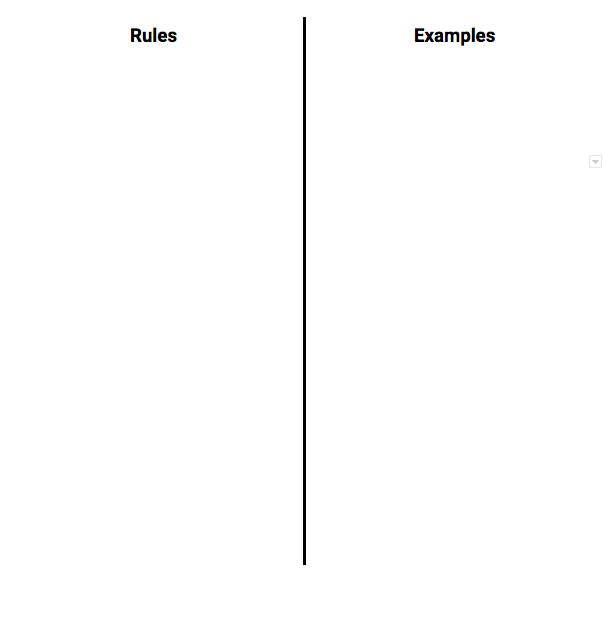
\includegraphics[width=\textwidth]{images/rules-examples}

\fi